% Options for packages loaded elsewhere
\PassOptionsToPackage{unicode}{hyperref}
\PassOptionsToPackage{hyphens}{url}
\PassOptionsToPackage{dvipsnames,svgnames,x11names}{xcolor}
%
\documentclass[
  letterpaper,
  DIV=11,
  numbers=noendperiod]{scrartcl}

\usepackage{amsmath,amssymb}
\usepackage{iftex}
\ifPDFTeX
  \usepackage[T1]{fontenc}
  \usepackage[utf8]{inputenc}
  \usepackage{textcomp} % provide euro and other symbols
\else % if luatex or xetex
  \usepackage{unicode-math}
  \defaultfontfeatures{Scale=MatchLowercase}
  \defaultfontfeatures[\rmfamily]{Ligatures=TeX,Scale=1}
\fi
\usepackage{lmodern}
\ifPDFTeX\else  
    % xetex/luatex font selection
\fi
% Use upquote if available, for straight quotes in verbatim environments
\IfFileExists{upquote.sty}{\usepackage{upquote}}{}
\IfFileExists{microtype.sty}{% use microtype if available
  \usepackage[]{microtype}
  \UseMicrotypeSet[protrusion]{basicmath} % disable protrusion for tt fonts
}{}
\makeatletter
\@ifundefined{KOMAClassName}{% if non-KOMA class
  \IfFileExists{parskip.sty}{%
    \usepackage{parskip}
  }{% else
    \setlength{\parindent}{0pt}
    \setlength{\parskip}{6pt plus 2pt minus 1pt}}
}{% if KOMA class
  \KOMAoptions{parskip=half}}
\makeatother
\usepackage{xcolor}
\setlength{\emergencystretch}{3em} % prevent overfull lines
\setcounter{secnumdepth}{-\maxdimen} % remove section numbering
% Make \paragraph and \subparagraph free-standing
\ifx\paragraph\undefined\else
  \let\oldparagraph\paragraph
  \renewcommand{\paragraph}[1]{\oldparagraph{#1}\mbox{}}
\fi
\ifx\subparagraph\undefined\else
  \let\oldsubparagraph\subparagraph
  \renewcommand{\subparagraph}[1]{\oldsubparagraph{#1}\mbox{}}
\fi

\usepackage{color}
\usepackage{fancyvrb}
\newcommand{\VerbBar}{|}
\newcommand{\VERB}{\Verb[commandchars=\\\{\}]}
\DefineVerbatimEnvironment{Highlighting}{Verbatim}{commandchars=\\\{\}}
% Add ',fontsize=\small' for more characters per line
\usepackage{framed}
\definecolor{shadecolor}{RGB}{241,243,245}
\newenvironment{Shaded}{\begin{snugshade}}{\end{snugshade}}
\newcommand{\AlertTok}[1]{\textcolor[rgb]{0.68,0.00,0.00}{#1}}
\newcommand{\AnnotationTok}[1]{\textcolor[rgb]{0.37,0.37,0.37}{#1}}
\newcommand{\AttributeTok}[1]{\textcolor[rgb]{0.40,0.45,0.13}{#1}}
\newcommand{\BaseNTok}[1]{\textcolor[rgb]{0.68,0.00,0.00}{#1}}
\newcommand{\BuiltInTok}[1]{\textcolor[rgb]{0.00,0.23,0.31}{#1}}
\newcommand{\CharTok}[1]{\textcolor[rgb]{0.13,0.47,0.30}{#1}}
\newcommand{\CommentTok}[1]{\textcolor[rgb]{0.37,0.37,0.37}{#1}}
\newcommand{\CommentVarTok}[1]{\textcolor[rgb]{0.37,0.37,0.37}{\textit{#1}}}
\newcommand{\ConstantTok}[1]{\textcolor[rgb]{0.56,0.35,0.01}{#1}}
\newcommand{\ControlFlowTok}[1]{\textcolor[rgb]{0.00,0.23,0.31}{#1}}
\newcommand{\DataTypeTok}[1]{\textcolor[rgb]{0.68,0.00,0.00}{#1}}
\newcommand{\DecValTok}[1]{\textcolor[rgb]{0.68,0.00,0.00}{#1}}
\newcommand{\DocumentationTok}[1]{\textcolor[rgb]{0.37,0.37,0.37}{\textit{#1}}}
\newcommand{\ErrorTok}[1]{\textcolor[rgb]{0.68,0.00,0.00}{#1}}
\newcommand{\ExtensionTok}[1]{\textcolor[rgb]{0.00,0.23,0.31}{#1}}
\newcommand{\FloatTok}[1]{\textcolor[rgb]{0.68,0.00,0.00}{#1}}
\newcommand{\FunctionTok}[1]{\textcolor[rgb]{0.28,0.35,0.67}{#1}}
\newcommand{\ImportTok}[1]{\textcolor[rgb]{0.00,0.46,0.62}{#1}}
\newcommand{\InformationTok}[1]{\textcolor[rgb]{0.37,0.37,0.37}{#1}}
\newcommand{\KeywordTok}[1]{\textcolor[rgb]{0.00,0.23,0.31}{#1}}
\newcommand{\NormalTok}[1]{\textcolor[rgb]{0.00,0.23,0.31}{#1}}
\newcommand{\OperatorTok}[1]{\textcolor[rgb]{0.37,0.37,0.37}{#1}}
\newcommand{\OtherTok}[1]{\textcolor[rgb]{0.00,0.23,0.31}{#1}}
\newcommand{\PreprocessorTok}[1]{\textcolor[rgb]{0.68,0.00,0.00}{#1}}
\newcommand{\RegionMarkerTok}[1]{\textcolor[rgb]{0.00,0.23,0.31}{#1}}
\newcommand{\SpecialCharTok}[1]{\textcolor[rgb]{0.37,0.37,0.37}{#1}}
\newcommand{\SpecialStringTok}[1]{\textcolor[rgb]{0.13,0.47,0.30}{#1}}
\newcommand{\StringTok}[1]{\textcolor[rgb]{0.13,0.47,0.30}{#1}}
\newcommand{\VariableTok}[1]{\textcolor[rgb]{0.07,0.07,0.07}{#1}}
\newcommand{\VerbatimStringTok}[1]{\textcolor[rgb]{0.13,0.47,0.30}{#1}}
\newcommand{\WarningTok}[1]{\textcolor[rgb]{0.37,0.37,0.37}{\textit{#1}}}

\providecommand{\tightlist}{%
  \setlength{\itemsep}{0pt}\setlength{\parskip}{0pt}}\usepackage{longtable,booktabs,array}
\usepackage{calc} % for calculating minipage widths
% Correct order of tables after \paragraph or \subparagraph
\usepackage{etoolbox}
\makeatletter
\patchcmd\longtable{\par}{\if@noskipsec\mbox{}\fi\par}{}{}
\makeatother
% Allow footnotes in longtable head/foot
\IfFileExists{footnotehyper.sty}{\usepackage{footnotehyper}}{\usepackage{footnote}}
\makesavenoteenv{longtable}
\usepackage{graphicx}
\makeatletter
\def\maxwidth{\ifdim\Gin@nat@width>\linewidth\linewidth\else\Gin@nat@width\fi}
\def\maxheight{\ifdim\Gin@nat@height>\textheight\textheight\else\Gin@nat@height\fi}
\makeatother
% Scale images if necessary, so that they will not overflow the page
% margins by default, and it is still possible to overwrite the defaults
% using explicit options in \includegraphics[width, height, ...]{}
\setkeys{Gin}{width=\maxwidth,height=\maxheight,keepaspectratio}
% Set default figure placement to htbp
\makeatletter
\def\fps@figure{htbp}
\makeatother

\KOMAoption{captions}{tableheading}
\makeatletter
\makeatother
\makeatletter
\makeatother
\makeatletter
\@ifpackageloaded{caption}{}{\usepackage{caption}}
\AtBeginDocument{%
\ifdefined\contentsname
  \renewcommand*\contentsname{Table of contents}
\else
  \newcommand\contentsname{Table of contents}
\fi
\ifdefined\listfigurename
  \renewcommand*\listfigurename{List of Figures}
\else
  \newcommand\listfigurename{List of Figures}
\fi
\ifdefined\listtablename
  \renewcommand*\listtablename{List of Tables}
\else
  \newcommand\listtablename{List of Tables}
\fi
\ifdefined\figurename
  \renewcommand*\figurename{Figure}
\else
  \newcommand\figurename{Figure}
\fi
\ifdefined\tablename
  \renewcommand*\tablename{Table}
\else
  \newcommand\tablename{Table}
\fi
}
\@ifpackageloaded{float}{}{\usepackage{float}}
\floatstyle{ruled}
\@ifundefined{c@chapter}{\newfloat{codelisting}{h}{lop}}{\newfloat{codelisting}{h}{lop}[chapter]}
\floatname{codelisting}{Listing}
\newcommand*\listoflistings{\listof{codelisting}{List of Listings}}
\makeatother
\makeatletter
\@ifpackageloaded{caption}{}{\usepackage{caption}}
\@ifpackageloaded{subcaption}{}{\usepackage{subcaption}}
\makeatother
\makeatletter
\@ifpackageloaded{tcolorbox}{}{\usepackage[skins,breakable]{tcolorbox}}
\makeatother
\makeatletter
\@ifundefined{shadecolor}{\definecolor{shadecolor}{rgb}{.97, .97, .97}}
\makeatother
\makeatletter
\makeatother
\makeatletter
\makeatother
\ifLuaTeX
  \usepackage{selnolig}  % disable illegal ligatures
\fi
\IfFileExists{bookmark.sty}{\usepackage{bookmark}}{\usepackage{hyperref}}
\IfFileExists{xurl.sty}{\usepackage{xurl}}{} % add URL line breaks if available
\urlstyle{same} % disable monospaced font for URLs
\hypersetup{
  pdftitle={Exercises week 36},
  colorlinks=true,
  linkcolor={blue},
  filecolor={Maroon},
  citecolor={Blue},
  urlcolor={Blue},
  pdfcreator={LaTeX via pandoc}}

\title{Exercises week 36}
\author{}
\date{}

\begin{document}
\maketitle
\ifdefined\Shaded\renewenvironment{Shaded}{\begin{tcolorbox}[interior hidden, breakable, enhanced, sharp corners, boxrule=0pt, borderline west={3pt}{0pt}{shadecolor}, frame hidden]}{\end{tcolorbox}}\fi

Python library import

\begin{Shaded}
\begin{Highlighting}[]
\ImportTok{import}\NormalTok{ numpy }\ImportTok{as}\NormalTok{ np}
\ImportTok{import}\NormalTok{ matplotlib.pyplot }\ImportTok{as}\NormalTok{ plt}
\ImportTok{from}\NormalTok{ sklearn.model\_selection }\ImportTok{import}\NormalTok{ train\_test\_split}

\KeywordTok{def}\NormalTok{ design\_poly\_n(x, n):}
\NormalTok{    X }\OperatorTok{=}\NormalTok{ np.zeros((}\BuiltInTok{len}\NormalTok{(x), n))}
\NormalTok{    X[:,}\DecValTok{0}\NormalTok{] }\OperatorTok{=} \DecValTok{1}
    \ControlFlowTok{for}\NormalTok{ i }\KeywordTok{in} \BuiltInTok{range}\NormalTok{(}\DecValTok{1}\NormalTok{, n):}
\NormalTok{        X[:,i] }\OperatorTok{=}\NormalTok{ (x}\OperatorTok{**}\NormalTok{i).T}
    \ControlFlowTok{return}\NormalTok{ X}
\end{Highlighting}
\end{Shaded}

R library import

\begin{Shaded}
\begin{Highlighting}[]
\FunctionTok{library}\NormalTok{(tidyverse)}
\FunctionTok{library}\NormalTok{(reticulate)}
\end{Highlighting}
\end{Shaded}

We start by generating data using the same code as last week.

\begin{Shaded}
\begin{Highlighting}[]
\NormalTok{np.random.seed(}\DecValTok{8392}\NormalTok{)}
\NormalTok{n }\OperatorTok{=} \DecValTok{100}
\CommentTok{\# Make data set.}
\NormalTok{x }\OperatorTok{=}\NormalTok{ np.linspace(}\OperatorTok{{-}}\DecValTok{3}\NormalTok{, }\DecValTok{3}\NormalTok{, n).reshape(}\OperatorTok{{-}}\DecValTok{1}\NormalTok{, }\DecValTok{1}\NormalTok{)}
\NormalTok{y }\OperatorTok{=}\NormalTok{ np.exp(}\OperatorTok{{-}}\NormalTok{x}\OperatorTok{**}\DecValTok{2}\NormalTok{) }\OperatorTok{+} \FloatTok{1.5} \OperatorTok{*}\NormalTok{ np.exp(}\OperatorTok{{-}}\NormalTok{(x}\OperatorTok{{-}}\DecValTok{2}\NormalTok{)}\OperatorTok{**}\DecValTok{2}\NormalTok{)}\OperatorTok{+}\NormalTok{ np.random.normal(}\DecValTok{0}\NormalTok{, }\FloatTok{0.1}\NormalTok{, x.shape)}

\NormalTok{X }\OperatorTok{=}\NormalTok{ design\_poly\_n(x, }\DecValTok{5}\NormalTok{)}
\NormalTok{np.random.seed(}\DecValTok{524}\NormalTok{)}
\NormalTok{X\_train, X\_test, y\_train, y\_test }\OperatorTok{=}\NormalTok{ train\_test\_split(X, y, test\_size}\OperatorTok{=}\FloatTok{0.2}\NormalTok{)}
\end{Highlighting}
\end{Shaded}

Then we scale input data by subtracting the mean of each column.

\begin{Shaded}
\begin{Highlighting}[]
\NormalTok{X\_colmeans }\OperatorTok{=}\NormalTok{ np.mean(X\_train, }\DecValTok{0}\NormalTok{)[}\DecValTok{1}\NormalTok{:]}

\CommentTok{\# without intercept}
\NormalTok{X\_train\_scaled }\OperatorTok{=}\NormalTok{ X\_train[:, }\DecValTok{1}\NormalTok{:] }\OperatorTok{{-}}\NormalTok{ X\_colmeans}
\NormalTok{X\_test\_scaled }\OperatorTok{=}\NormalTok{ X\_test[:, }\DecValTok{1}\NormalTok{:] }\OperatorTok{{-}}\NormalTok{ X\_colmeans}
\NormalTok{y\_scaler }\OperatorTok{=}\NormalTok{ np.mean(y\_train)}
\NormalTok{y\_train\_scaled }\OperatorTok{=}\NormalTok{ y\_train }\OperatorTok{{-}}\NormalTok{ y\_scaler}
\end{Highlighting}
\end{Shaded}

First we fit with ordinary least squares

\begin{Shaded}
\begin{Highlighting}[]
\NormalTok{Bhat }\OperatorTok{=}\NormalTok{ np.linalg.inv(X\_train\_scaled.T }\OperatorTok{@}\NormalTok{ X\_train\_scaled) }\OperatorTok{@}\NormalTok{ X\_train\_scaled.T }\OperatorTok{@}\NormalTok{ y\_train\_scaled}

\BuiltInTok{print}\NormalTok{(}\StringTok{"Beta:"}\NormalTok{, Bhat.T)}
\end{Highlighting}
\end{Shaded}

\begin{verbatim}
Beta: [[ 0.44343093 -0.00864978 -0.0346039  -0.00467165]]
\end{verbatim}

\begin{Shaded}
\begin{Highlighting}[]
\NormalTok{ytilde\_train }\OperatorTok{=}\NormalTok{ X\_train\_scaled }\OperatorTok{@}\NormalTok{ Bhat }\OperatorTok{+}\NormalTok{ y\_scaler}
\NormalTok{intercept }\OperatorTok{=}\NormalTok{ y\_scaler }\OperatorTok{{-}}\NormalTok{ X\_colmeans }\OperatorTok{@}\NormalTok{ Bhat}

\NormalTok{MSE\_OLS\_train }\OperatorTok{=} \BuiltInTok{sum}\NormalTok{((y\_train }\OperatorTok{{-}}\NormalTok{ ytilde\_train)}\OperatorTok{**}\DecValTok{2}\NormalTok{) }\OperatorTok{/} \BuiltInTok{len}\NormalTok{(y\_train)}
\BuiltInTok{print}\NormalTok{(}\StringTok{"training data MSE:"}\NormalTok{, MSE\_OLS\_train)}
\end{Highlighting}
\end{Shaded}

\begin{verbatim}
training data MSE: [0.03319703]
\end{verbatim}

\begin{Shaded}
\begin{Highlighting}[]
\NormalTok{ytilde\_test }\OperatorTok{=}\NormalTok{ X\_test\_scaled }\OperatorTok{@}\NormalTok{ Bhat }\OperatorTok{+}\NormalTok{ y\_scaler }
\NormalTok{MSE\_OLS\_test }\OperatorTok{=} \BuiltInTok{sum}\NormalTok{((y\_test }\OperatorTok{{-}}\NormalTok{ ytilde\_test)}\OperatorTok{**}\DecValTok{2}\NormalTok{) }\OperatorTok{/} \BuiltInTok{len}\NormalTok{(y\_test)}
\BuiltInTok{print}\NormalTok{(}\StringTok{"test data MSE:"}\NormalTok{, MSE\_OLS\_test)}
\end{Highlighting}
\end{Shaded}

\begin{verbatim}
test data MSE: [0.03824773]
\end{verbatim}

And then fit the same data with ridge regression

\begin{Shaded}
\begin{Highlighting}[]
\CommentTok{\# define some functions for convenience}
\KeywordTok{def}\NormalTok{ get\_ridge\_beta(X, y, lmbda):}
\NormalTok{    p }\OperatorTok{=}\NormalTok{ X.shape[}\DecValTok{1}\NormalTok{]}
\NormalTok{    I }\OperatorTok{=}\NormalTok{ np.eye(p,p)}
    
    \ControlFlowTok{return}\NormalTok{ np.linalg.pinv(X.T }\OperatorTok{@}\NormalTok{ X }\OperatorTok{+}\NormalTok{ (lmbda }\OperatorTok{*}\NormalTok{ I)) }\OperatorTok{@}\NormalTok{ X.T }\OperatorTok{@}\NormalTok{ y}

\KeywordTok{def}\NormalTok{ predict(X, Beta, scaler }\OperatorTok{=} \DecValTok{0}\NormalTok{):}
    \ControlFlowTok{return}\NormalTok{ X }\OperatorTok{@}\NormalTok{ Beta }\OperatorTok{+}\NormalTok{ scaler}

\KeywordTok{def}\NormalTok{ get\_intercept(X, Beta, scaler):}
    \ControlFlowTok{return}\NormalTok{ scaler }\OperatorTok{{-}}\NormalTok{ np.mean(X, }\DecValTok{0}\NormalTok{) }\OperatorTok{@}\NormalTok{ Beta}

\KeywordTok{def}\NormalTok{ MSE(y, ytilde):}
    \ControlFlowTok{return} \BuiltInTok{sum}\NormalTok{((y }\OperatorTok{{-}}\NormalTok{ ytilde)}\OperatorTok{**}\DecValTok{2}\NormalTok{) }\OperatorTok{/} \BuiltInTok{len}\NormalTok{(y)}
\end{Highlighting}
\end{Shaded}

\begin{Shaded}
\begin{Highlighting}[]
\NormalTok{lambdas }\OperatorTok{=} \DecValTok{10}\OperatorTok{**}\NormalTok{np.arange(}\OperatorTok{{-}}\DecValTok{4}\NormalTok{, }\DecValTok{1}\NormalTok{, dtype }\OperatorTok{=} \BuiltInTok{float}\NormalTok{)}
\NormalTok{MSE\_train }\OperatorTok{=}\NormalTok{ np.zeros(}\BuiltInTok{len}\NormalTok{(lambdas))}
\NormalTok{MSE\_test }\OperatorTok{=}\NormalTok{ np.zeros(}\BuiltInTok{len}\NormalTok{(lambdas))}

\ControlFlowTok{for}\NormalTok{ i }\KeywordTok{in} \BuiltInTok{range}\NormalTok{(}\BuiltInTok{len}\NormalTok{(lambdas)):}
\NormalTok{    ridge\_beta }\OperatorTok{=}\NormalTok{ get\_ridge\_beta(X\_train\_scaled, y\_train\_scaled, }
\NormalTok{                                lambdas.item(i))}
    
\NormalTok{    y\_ridge\_train }\OperatorTok{=}\NormalTok{ predict(X\_train\_scaled, ridge\_beta, y\_scaler)}
\NormalTok{    y\_ridge\_test }\OperatorTok{=}\NormalTok{ predict(X\_test\_scaled, ridge\_beta, y\_scaler)}
    
\NormalTok{    MSE\_tr }\OperatorTok{=}\NormalTok{ MSE(y\_train, y\_ridge\_train)}
\NormalTok{    MSE\_te }\OperatorTok{=}\NormalTok{ MSE(y\_test, y\_ridge\_test)}
\NormalTok{    MSE\_train[i] }\OperatorTok{=}\NormalTok{ MSE\_tr}
\NormalTok{    MSE\_test[i] }\OperatorTok{=}\NormalTok{ MSE\_te}

\NormalTok{MSE\_train}
\end{Highlighting}
\end{Shaded}

\begin{verbatim}
array([0.03319703, 0.03319703, 0.03319704, 0.03319765, 0.03325636])
\end{verbatim}

\begin{Shaded}
\begin{Highlighting}[]
\NormalTok{MSE\_test}
\end{Highlighting}
\end{Shaded}

\begin{verbatim}
array([0.03824774, 0.03824787, 0.03824919, 0.03826286, 0.03844413])
\end{verbatim}

\begin{Shaded}
\begin{Highlighting}[]
\NormalTok{plt.plot(lambdas, MSE\_train, }\StringTok{"b{-}"}\NormalTok{, label }\OperatorTok{=} \StringTok{"training data"}\NormalTok{)}
\NormalTok{plt.plot(lambdas, MSE\_test, }\StringTok{"b{-}."}\NormalTok{, label }\OperatorTok{=} \StringTok{"test data"}\NormalTok{)}
\NormalTok{plt.xlabel(}\StringTok{"lambda"}\NormalTok{)}
\NormalTok{plt.ylabel(}\StringTok{"MSE"}\NormalTok{)}
\NormalTok{plt.legend()}
\NormalTok{plt.show()}
\end{Highlighting}
\end{Shaded}

\begin{figure}[H]

{\centering 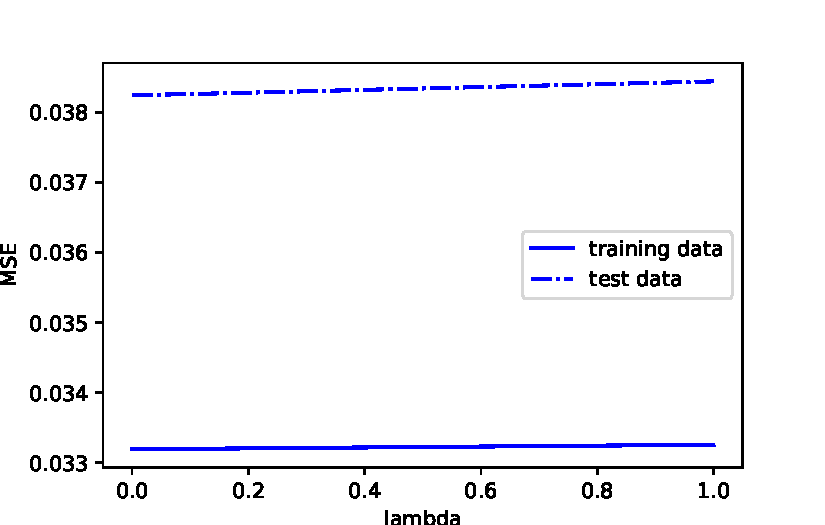
\includegraphics{w36-exercises_files/figure-pdf/unnamed-chunk-7-1.pdf}

}

\caption{MSE as function of lambda for a ridge regression with
predictors up to a 5th degree polynomial.}

\end{figure}

We can see that the MSE increases with increasing \(\lambda\) for both
training and test data.

Finally, we do the same for multiple maximum polynomial degrees: 5, 10
and 15.

\begin{Shaded}
\begin{Highlighting}[]
\KeywordTok{def}\NormalTok{ ridge\_test\_lambdas(X, y, lambdas):}
    
    \CommentTok{\#\# Split and scale data}
\NormalTok{    X\_train, X\_test, y\_train, y\_test }\OperatorTok{=}\NormalTok{ train\_test\_split(X, y, test\_size}\OperatorTok{=}\FloatTok{0.2}\NormalTok{)}
\NormalTok{    X\_colmeans }\OperatorTok{=}\NormalTok{ np.mean(X\_train, }\DecValTok{0}\NormalTok{)[}\DecValTok{1}\NormalTok{:]}

    \CommentTok{\# without intercept}
\NormalTok{    X\_train\_scaled }\OperatorTok{=}\NormalTok{ X\_train[:, }\DecValTok{1}\NormalTok{:] }\OperatorTok{{-}}\NormalTok{ X\_colmeans}
\NormalTok{    X\_test\_scaled }\OperatorTok{=}\NormalTok{ X\_test[:, }\DecValTok{1}\NormalTok{:] }\OperatorTok{{-}}\NormalTok{ X\_colmeans}
\NormalTok{    y\_scaler }\OperatorTok{=}\NormalTok{ np.mean(y\_train)}
\NormalTok{    y\_train\_scaled }\OperatorTok{=}\NormalTok{ y\_train }\OperatorTok{{-}}\NormalTok{ y\_scaler}
    
    \CommentTok{\#\# Fit models for different lambdas}
\NormalTok{    MSE\_train }\OperatorTok{=}\NormalTok{ np.zeros(}\BuiltInTok{len}\NormalTok{(lambdas))}
\NormalTok{    MSE\_test }\OperatorTok{=}\NormalTok{ np.zeros(}\BuiltInTok{len}\NormalTok{(lambdas))}
    
    \ControlFlowTok{for}\NormalTok{ i }\KeywordTok{in} \BuiltInTok{range}\NormalTok{(}\BuiltInTok{len}\NormalTok{(lambdas)):}
\NormalTok{        ridge\_beta }\OperatorTok{=}\NormalTok{ get\_ridge\_beta(X\_train\_scaled, y\_train\_scaled,}
\NormalTok{                                    lambdas.item(i))}

\NormalTok{        y\_ridge\_train }\OperatorTok{=}\NormalTok{ predict(X\_train\_scaled, ridge\_beta, y\_scaler)}
\NormalTok{        y\_ridge\_test }\OperatorTok{=}\NormalTok{ predict(X\_test\_scaled, ridge\_beta, y\_scaler)}
        
\NormalTok{        MSE\_tr }\OperatorTok{=}\NormalTok{ MSE(y\_train, y\_ridge\_train)}
\NormalTok{        MSE\_te }\OperatorTok{=}\NormalTok{ MSE(y\_test, y\_ridge\_test)}
\NormalTok{        MSE\_train[i] }\OperatorTok{=}\NormalTok{ MSE\_tr}
\NormalTok{        MSE\_test[i] }\OperatorTok{=}\NormalTok{ MSE\_te}
    
    \ControlFlowTok{return}\NormalTok{ [MSE\_train, MSE\_test]}
\end{Highlighting}
\end{Shaded}

\begin{Shaded}
\begin{Highlighting}[]
\NormalTok{polys }\OperatorTok{=}\NormalTok{ [}\DecValTok{5}\NormalTok{, }\DecValTok{10}\NormalTok{, }\DecValTok{15}\NormalTok{]}
\NormalTok{lambdas }\OperatorTok{=} \DecValTok{10}\OperatorTok{**}\NormalTok{np.arange(}\OperatorTok{{-}}\DecValTok{4}\NormalTok{, }\DecValTok{1}\NormalTok{, dtype }\OperatorTok{=} \BuiltInTok{float}\NormalTok{)}
\NormalTok{MSE\_train\_p }\OperatorTok{=}\NormalTok{ np.zeros((}\BuiltInTok{len}\NormalTok{(lambdas), }\BuiltInTok{len}\NormalTok{(polys)))}
\NormalTok{MSE\_test\_p }\OperatorTok{=}\NormalTok{ np.zeros((}\BuiltInTok{len}\NormalTok{(lambdas), }\BuiltInTok{len}\NormalTok{(polys)))}

\ControlFlowTok{for}\NormalTok{ j }\KeywordTok{in} \BuiltInTok{range}\NormalTok{(}\BuiltInTok{len}\NormalTok{(polys)):}
\NormalTok{    X }\OperatorTok{=}\NormalTok{ design\_poly\_n(x, polys[j])}
\NormalTok{    np.random.seed(}\DecValTok{524}\NormalTok{)}
\NormalTok{    MSE\_train, MSE\_test }\OperatorTok{=}\NormalTok{ ridge\_test\_lambdas(X, y, lambdas)}
\NormalTok{    MSE\_train\_p[:,j] }\OperatorTok{=}\NormalTok{ MSE\_train}
\NormalTok{    MSE\_test\_p[:,j] }\OperatorTok{=}\NormalTok{ MSE\_test}
\end{Highlighting}
\end{Shaded}

Hand over to R

\begin{Shaded}
\begin{Highlighting}[]
\NormalTok{train\_data }\OtherTok{\textless{}{-}} \FunctionTok{as.data.frame}\NormalTok{(py}\SpecialCharTok{$}\NormalTok{MSE\_train\_p)}
\NormalTok{test\_data }\OtherTok{\textless{}{-}} \FunctionTok{as.data.frame}\NormalTok{(py}\SpecialCharTok{$}\NormalTok{MSE\_test\_p)}
\FunctionTok{names}\NormalTok{(train\_data) }\OtherTok{\textless{}{-}} \FunctionTok{names}\NormalTok{(test\_data) }\OtherTok{\textless{}{-}} \FunctionTok{paste0}\NormalTok{(py}\SpecialCharTok{$}\NormalTok{polys)}

\NormalTok{train\_data}\SpecialCharTok{$}\NormalTok{dat }\OtherTok{\textless{}{-}} \StringTok{"training"}
\NormalTok{test\_data}\SpecialCharTok{$}\NormalTok{dat }\OtherTok{\textless{}{-}} \StringTok{"test"}

\FunctionTok{rbind}\NormalTok{(train\_data, test\_data) }\SpecialCharTok{\%\textgreater{}\%}
    \FunctionTok{cbind}\NormalTok{(}\AttributeTok{lmb =}\NormalTok{ py}\SpecialCharTok{$}\NormalTok{lambdas) }\SpecialCharTok{\%\textgreater{}\%}
    \FunctionTok{pivot\_longer}\NormalTok{(}\SpecialCharTok{{-}}\FunctionTok{c}\NormalTok{(dat, lmb)) }\SpecialCharTok{\%\textgreater{}\%}
    \FunctionTok{ggplot}\NormalTok{(}\FunctionTok{aes}\NormalTok{(lmb, value, }\AttributeTok{lty =}\NormalTok{ dat)) }\SpecialCharTok{+}
    \FunctionTok{geom\_line}\NormalTok{() }\SpecialCharTok{+}
    \FunctionTok{facet\_wrap}\NormalTok{(}\SpecialCharTok{\textasciitilde{}}\FunctionTok{as.numeric}\NormalTok{(name),}\AttributeTok{nrow =} \DecValTok{3}\NormalTok{, }\AttributeTok{scales =} \StringTok{"free\_y"}\NormalTok{) }\SpecialCharTok{+}
    \FunctionTok{labs}\NormalTok{(}\AttributeTok{x =} \FunctionTok{expression}\NormalTok{(}\FunctionTok{paste}\NormalTok{(lambda)),}
         \AttributeTok{y =} \StringTok{"MSE"}\NormalTok{,}
         \AttributeTok{linetype =} \StringTok{"data"}\NormalTok{) }\SpecialCharTok{+}
    \FunctionTok{theme\_bw}\NormalTok{() }\SpecialCharTok{+}
    \FunctionTok{scale\_x\_log10}\NormalTok{()}
\end{Highlighting}
\end{Shaded}

\begin{figure}[H]

{\centering 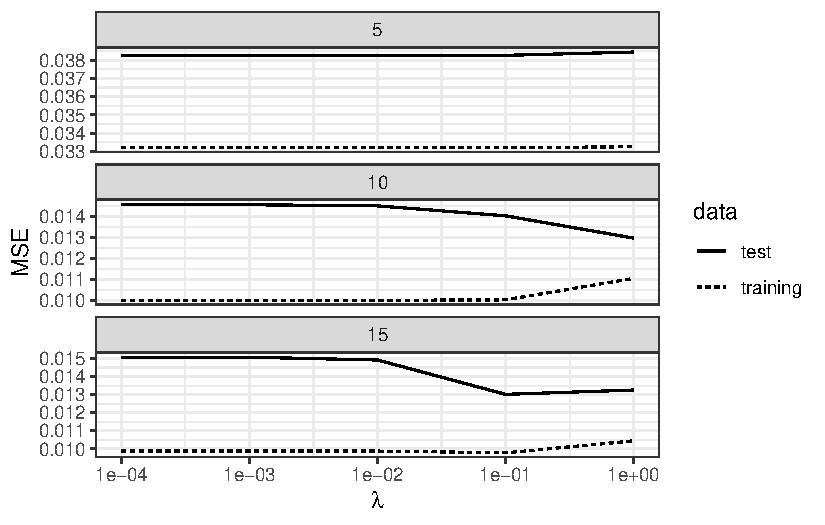
\includegraphics{w36-exercises_files/figure-pdf/unnamed-chunk-10-3.pdf}

}

\caption{Mean square error for different as a function of \(\lambda\)
for fits with predictors of polynomial degree up to 5, 10 and 15. Note
individual Y-axis on each plot to emphasize patterns in the data.}

\end{figure}

In general, training data MSE increases with increasing \(\lambda\). It
seems that the model performs best on the test data when
\(\lambda \ge 0.1\) for the higher polynomial degrees, showing that the
ridge regression could reduce overfitting for this data.



\end{document}
